% arara: xelatex
% arara: biber
% arara: xelatex
% arara: xelatex

\documentclass[
% handout,
]{beamer}

%\usepackage{fontspec}
%\setsansfont{Helvetica Neue}

\usepackage[backend=biber, doi=false]{biblatex}
\addbibresource{refs.bib}

\usepackage{xspace}
\newcommand\st{SSA-Tool\xspace}

\usepackage{menukeys}
\usepackage{style}
\usepackage{smcm-cosc-listings}

\tikzset{
  invisible/.style={opacity=0},
  visible on/.style={alt={#1{}{invisible}}},
  alt/.code args={<#1>#2#3}{%
    \alt<#1>{\pgfkeysalso{#2}}{\pgfkeysalso{#3}} % \pgfkeysalso doesn't change the path
  },
  marked on/.style={alt=#1{}{marked}},
}

\lstdefinestyle{pyhl}{
  keywordstyle=\color{blue}\bfseries,
}
\lstdefinestyle{pystep}{
  language=Python,
  basicstyle=\color{black!40}\ttfamily,
  keywordstyle=\color{blue!40}\bfseries,
  moredelim=**[is][\only<+>{\color{black}\lstset{style=pyhl}}]{@}{@},
  moredelim=**[is][\only<.>{\color{black}\lstset{style=pyhl}}]{@@}{@@},
}

\title{\st}
\subtitle{A Utility for the Creation and Evaluation of Self-Stabilizing Algorithms}
\author{Sean Allred}
\date{May 6, 2014}
\institute[SMCM]{%
  St. Mary's College \\[1ex] % TODO 'of md' necessary?
  Department of Mathematics \\
  and Computer Science}
\titlegraphic{
\includegraphics[height=.15\textheight]{../poster/seal}}

\begin{document}
\maketitle

\section{Introduction}
\begin{frame}
  \frametitle{Introduction}
  \begin{block}{General}
    \begin{itemize}[<+->]
    \item an entire family of distributed algorithms
    \item most effectively applied to connected, \emph{sparse} networks
    \item self-stabilizing\slash fault-tolerant
    \end{itemize}
  \end{block}
  \begin{block}<4->{Qualities}
    \begin{itemize}[<+->]
    \item each node is semi-autonomous
    \item very parallelizable
    \item execution is sometimes controlled by a central daemon
    \end{itemize}
  \end{block}
\end{frame}

\subsection{History}
\begin{frame}
  \frametitle{History}
  \begin{description}[<+->]
  \item[\citeyear{dew:sem}] Put forward by \citeauthor{dew:sem} in
    \citetitle{dew:sem}
  \item[\citeyear{lamport}] \citeauthor{lamport} draws attention to the above,
    calling~it \enquote{Dijkstra's most brilliant work}
  \end{description}
\end{frame}

\subsection{Definition}
\begin{frame}
  \frametitle{Definition}
  \begin{block}{Functions of a Node and its Neighbors}
    \begin{description}
    \item[predicate]<2- | alert@3> $\Function[f]{v, N(\!v)}{\SetBoolean}$
    \item[move]<2-> new state for $v$
    \end{description}
  \end{block}
  \begin{block}{Collections of Rules}
    \begin{description}
    \item[rule]<4-> $\Function[R]{P}{M}$
    \item[algorithm]<4-> $\Set{\QuickSequence{R}}$
    \end{description}
  \end{block}
\end{frame}

\subsection{Running}
\begin{frame}
  \frametitle{Running an Algorithm}
  \begin{enumerate}[<+->]
  \item System received in an arbitrary state \label{step:receive}
  \item Central daemon chooses \enquote*{privileged} node $p$
  \item $p$ makes its move
  \item Process repeats; continuing to step~\autoref{step:receive}
  \end{enumerate}
\end{frame}

\subsection{Example}
\begin{frame}[fragile]
  \frametitle{Example \Dash Maximal Independent Set}
  \begin{description}[<+->]
  \item[independent set] a set of vertices in a graph such that no two
    vertices in the set are adjacent
  \item[maximal independent set] an independent set that is not the
    subset of any other independent set
  \end{description}    
\end{frame}
% definitions
\begin{frame}[fragile]
  \frametitle{Example \Dash Maximal Independent Set}
\begin{lstlisting}[language=ssa]
local $\operatorname{marked}$

privilege ENTER
  if unmarked and neighbors unmarked
  then mark

privilege LEAVE
  if marked and neighbor marked
  then unmark
\end{lstlisting}
\end{frame}
% both privileges
\begin{frame}
  \frametitle{Example \Dash Maximal Independent Set \qquad $t=\arabic{slideinframe}$}
  \centering
    \begin{tikzpicture}
      \node[graph vertex, marked] (1) at (0 , 3) {$v_1$};
      \node[graph vertex,       ] (2) at (0 , 6) {$v_2$};
      \node[graph vertex,       ] (3) at (3 , 3) {$v_3$};
      \node[graph vertex, alt=<1-2>{marked}{}] (4) at (3 , 6) {$v_4$};
      \node[graph vertex, alt=<2-3>{marked}{}] (5) at (5 , 8) {$v_5$};

      \graph {
        (1) -- (3) -- (4) -- (2) --[bend left] (5),
        (1) -- (2),
        (1) -- (4),
        (3) --[bend right] (5)
      };
  \end{tikzpicture}
\end{frame}

\section{Logic}
\begin{frame}
  \frametitle{Logical Representation}
  \begin{block}<1->{Mathematics is\dots}
    \begin{itemize}
    \item<1-> difficult to parse
    \item<2-> potentially ambiguous
      % properties and functions have no implicit difference
    \item<3-> very dense when written formally
    \end{itemize}
  \end{block}
  \begin{block}<5->{A New System?}
    To overcome these obstacles, it is clear that \\ a new system is required.
  \end{block}
\end{frame}

\subsection{Overview}
\begin{frame}
  \frametitle{Logical Representation}
  \begin{block}{Requirements}
    \begin{itemize}[<+->]
    \item accessible
    \item extensible
    \item sensible
    \end{itemize}
  \end{block}
  \begin{block}<+->{Implementation}
    \begin{description}[<+->]
    \item[predicates]<.-> Python snippets
    \item[moves] Python snippets
    \item[algorithms] \alert<+->{YAML} relationship serialization
    \end{description}
  \end{block}
\end{frame}

\subsection{Implementation}
\begin{frame}
  \frametitle{Logical Representation}
  \begin{block}{Why YAML?}
    \begin{itemize}[<+->]
    \item plain-text
    \item quickly growing standard
    \item manual editing is feasible
    \item many parsers available
    \end{itemize}
  \end{block}
\end{frame}

\subsection{Example}
\begin{frame}[fragile]
  \frametitle{Example \Dash Maximal Independent Set}
\begin{lstlisting}[style=myyaml]
--- !Predicate
name: node should mark
filename: enter.py
--- !Predicate
name: node should unmark
filename: leave.py
\end{lstlisting}
\end{frame}
\begin{frame}[fragile]
  \frametitle{Example \Dash Maximal Independent Set}
  \directory{ind-set.ssax/predicates/enter.py}
  \vspace{1ex}
\begin{lstlisting}[style=mypy]
  marked = v['marked']
  neighbor_marked = \
    any(map(lambda n: n['marked'], N))
  return not (marked or neighbor_marked)
\end{lstlisting}

\end{frame}
\begin{frame}[fragile]
  \frametitle{Example \Dash Maximal Independent Set}
\begin{lstlisting}[style=myyaml]
--- !Move
name: mark
filename: mark.py
--- !Move
name: unmark
filename: unmark.py
\end{lstlisting}
\end{frame}
\begin{frame}[fragile]
  \frametitle{Example \Dash Maximal Independent Set}
  \directory{ind-set.ssax/moves/mark.py}
  \vspace{1ex}
\begin{lstlisting}[style=mypy]
  v['marked'] = True
\end{lstlisting}
\end{frame}

\begin{frame}[fragile]
  \frametitle{Example \Dash Maximal Independent Set}
\begin{lstlisting}[style=myyaml]
--- !Algorithm
name: Independent Set
rules:
  - !Rule
    predicate: enter
    moves: [ mark ]
  - !Rule
    predicate: leave
    moves: [ unmark ]
\end{lstlisting}
\end{frame}

\subsection{Execution}
\begin{frame}
  \frametitle{Execution}
  \begin{enumerate}[<+->]
  \item find privileged nodes
  \item select random rule
  \item select random move
  \item execute move
  \item calculate delta
  \item add delta to \texttt{AnimatedGraph}
  \end{enumerate}
\end{frame}

\begin{frame}[fragile]
  \frametitle{Execution \Dash Finding Privileged Nodes}
\begin{lstlisting}[style=pystep]
p_nodes = dict()
@for node in graph:@
  @for rule in self.rules:@
    @if rule.applies_to(v, N(v)):@
      @p_nodes[node] += rule@
@if not p_nodes:@
    @@break@@
\end{lstlisting}
\end{frame}
\begin{frame}[fragile]
  \frametitle{Execution \Dash Applying Rules}
\begin{lstlisting}[style=pystep]
@node = rand(p_nodes)@
@@rule = rand(p_nodes[node])@@
@log  = rule.apply_to(graph, node)@
@history.append(log)@
\end{lstlisting}
\end{frame}

\section{Interface}
\begin{frame}
  \frametitle{Graphical Interface}
  \begin{block}{Why is it Necessary?}
    \begin{itemize}[<+->]
    \item Not all mathematicians are computer scientists
    \item Not all computer scientists are programmers
    \end{itemize}
  \end{block}
  \begin{block}<+->{Requirements}
    \begin{itemize}[<+->]
    \item<.-> Portable and cross-platform
    \item Supportive of the core features of \st
    \item Minimizes interfacing with underlying structure
    \item Representative of mathematical definitions
    \end{itemize}
  \end{block}
\end{frame}

\subsection{Bundles}
\begin{frame}
  \frametitle{Graphical Interface}
  \centering
  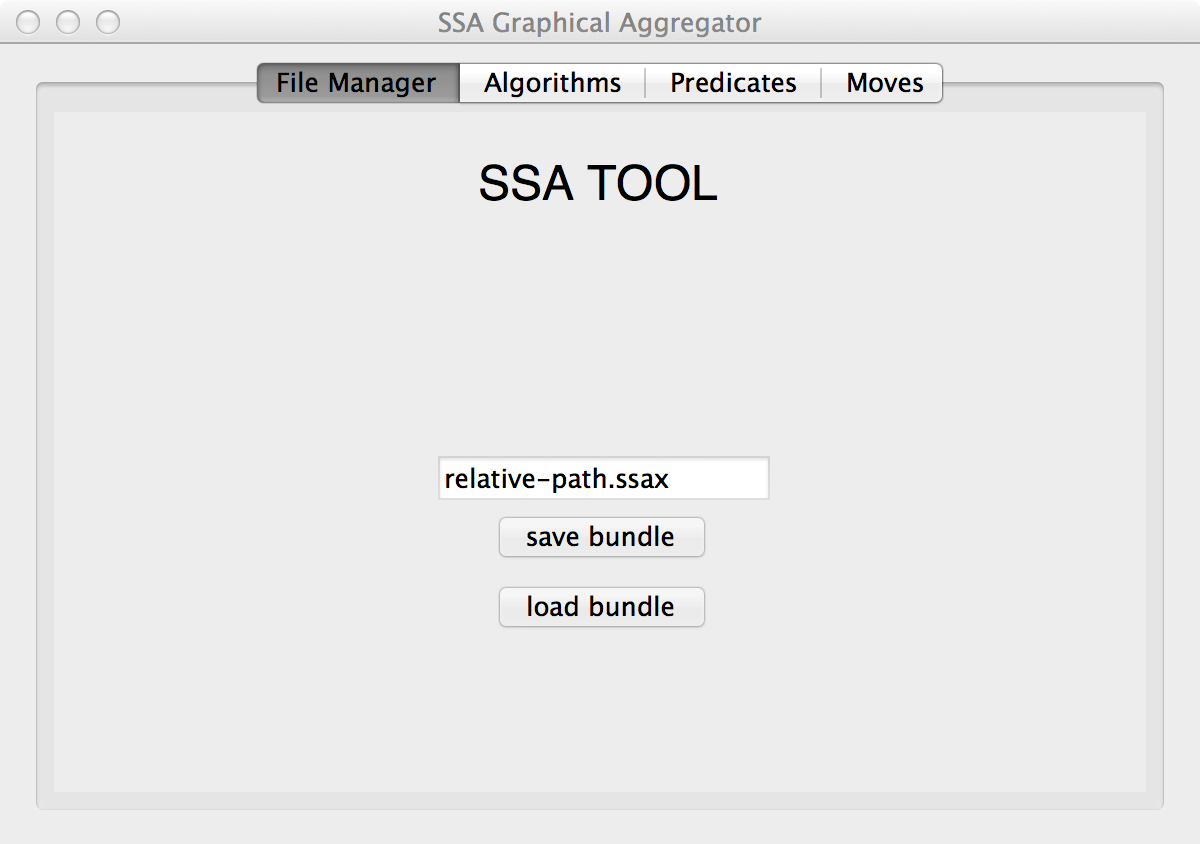
\includegraphics[width=\textwidth]{../figs/3-2}
\end{frame}

\tikzset{
  hlbox/.style={
    red, ultra thick, rounded corners
  }
}
\subsection{Algorithms}
\begin{frame}
  \frametitle{Graphical Interface}
  \centering
  \begin{tikzpicture}
    \node[anchor=south west, inner sep=0, opacity=1] (image) at (0, 0)
      {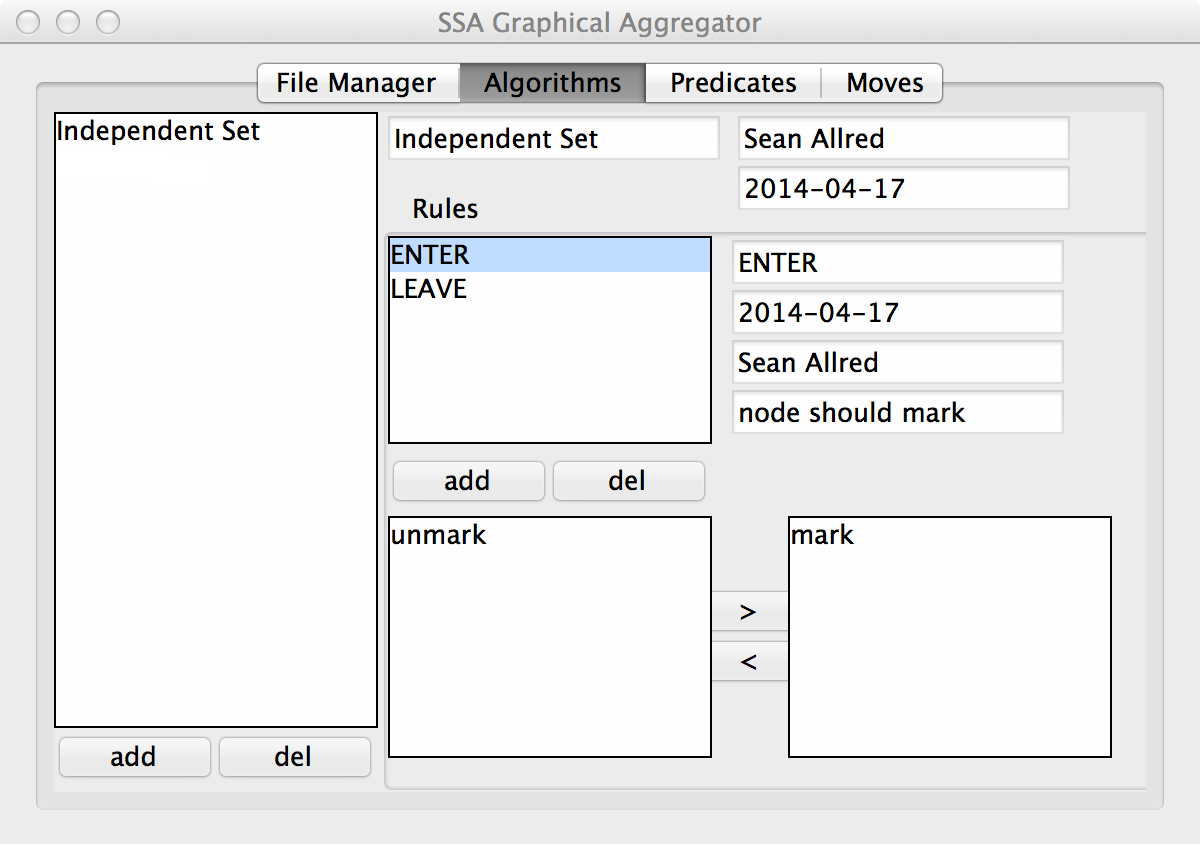
\includegraphics[width=\textwidth]{../figs/4}};

      \begin{scope}[x={(image.south east)}, y={(image.north west)}]
        %\draw[help lines,xstep=.1,ystep=.1] (0,0) grid (1,1);
        %\foreach \x in {0,1,...,10} { \node [anchor=north] at (\x/10,0) {\small \x}; }
        %\foreach \y in {0,1,...,10} { \node [anchor=east] at (0,\y/10) {\small \y}; }

        \coordinate  (1) at (0.035, 0.880);
        \coordinate  (2) at (0.325, 0.060);

        \coordinate  (3) at (0.325, 0.870);
        \coordinate  (4) at (0.900, 0.870);
        \coordinate  (5) at (0.900, 0.740);
        \coordinate  (6) at (0.605, 0.740);
        \coordinate  (7) at (0.605, 0.800);
        \coordinate  (8) at (0.325, 0.800);

        \coordinate  (9) at (0.315, 0.775);
        \coordinate (10) at (0.425, 0.775);
        \coordinate (11) at (0.475, 0.740);
        \coordinate (12) at (0.895, 0.740);
        \coordinate (13) at (0.895, 0.475);
        \coordinate (14) at (0.605, 0.475);
        \coordinate (15) at (0.605, 0.390);
        \coordinate (16) at (0.315, 0.390);

        \coordinate (17) at (0.935, 0.740);
        \coordinate (18) at (0.935, 0.090);
        \coordinate (19) at (0.315, 0.090);

        \foreach \coord in {1,...,19} {
        % \draw[red,fill=red] (\coord) circle (1pt) node[right,black] {\tiny\tt\bf\coord};
        }

        \draw[hlbox, visible on=<2>] (1) rectangle (2);
        \draw[hlbox, visible on=<3>] (3) -- (4) -- (5) -- (6) -- (7) -- (8) -- cycle;
        \draw[hlbox, visible on=<4>] (9) -- (10) -- (11) -- (12) -- (13) -- (14) -- (15) -- (16) -- cycle;
        \draw[hlbox, visible on=<5>] (9) -- (10) -- (11) -- (17) -- (18) -- (19) -- cycle;
      \end{scope}
  \end{tikzpicture}

\end{frame}

\subsection{Predicates\slash Moves}
\begin{frame}
  \frametitle{Graphical Interface}
  \centering
\begin{tikzpicture}
    \node[anchor=south west, inner sep=0, opacity=1] (image) at (0, 0)
      {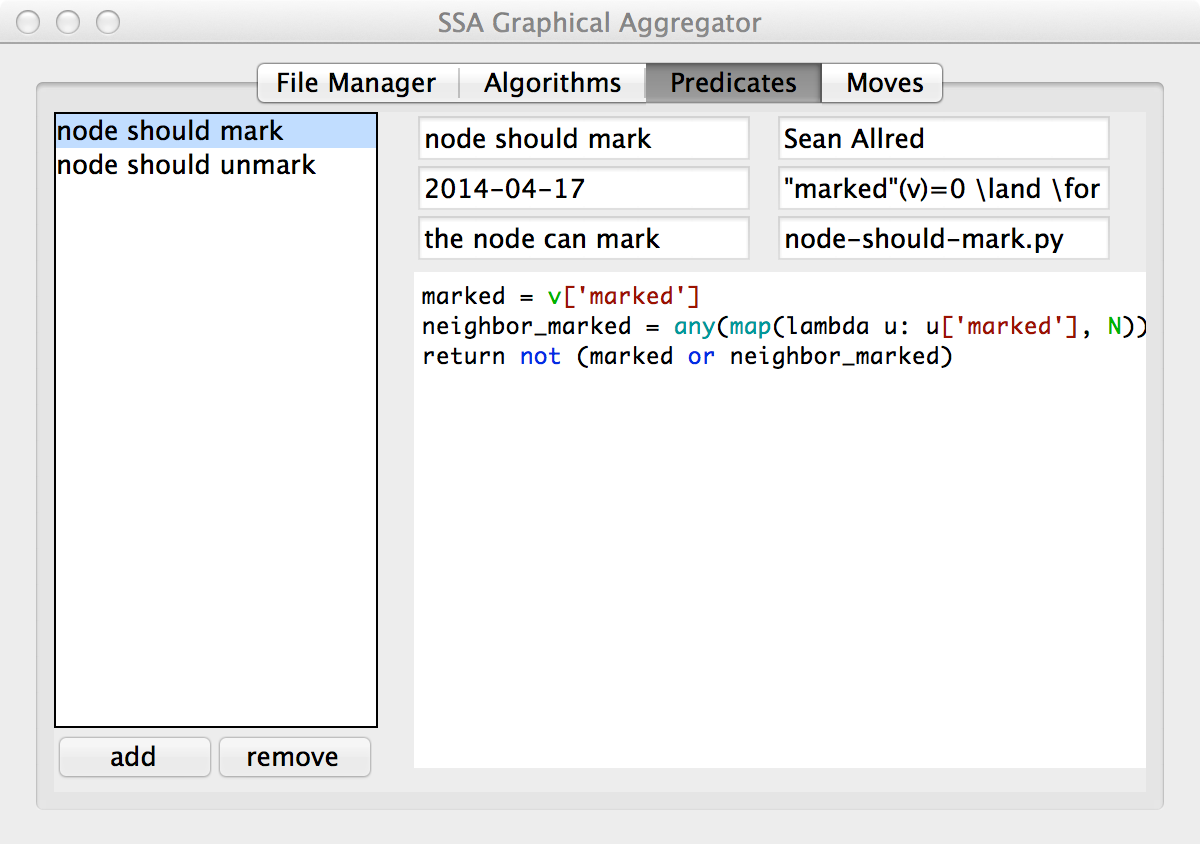
\includegraphics[width=\textwidth]{../figs/2}};

      \begin{scope}[x={(image.south east)}, y={(image.north west)}]
        %\draw[help lines,xstep=.1,ystep=.1] (0,0) grid (1,1);
        %\foreach \x in {0,1,...,10} { \node [anchor=north] at (\x/10,0) {\small \x}; }
        %\foreach \y in {0,1,...,10} { \node [anchor=east] at (0,\y/10) {\small \y}; }

        \coordinate (1) at (0.035, 0.880);
        \coordinate (2) at (0.325, 0.060);

        \coordinate (3) at (0.340, 0.875);
        \coordinate (4) at (0.934, 0.680);
        \coordinate (5) at (0.335, 0.690);
        \coordinate (6) at (0.964, 0.075);

        \foreach \coord in {5,...,6} {
          %\draw[red,fill=red] (\coord) circle (1pt) node[right,black] {\tiny\tt\bf\coord};
        }

        \draw[hlbox, visible on=<2>] (1) rectangle (2);
        \draw[hlbox, visible on=<3>] (3) rectangle (4);
        \draw[hlbox, visible on=<4>] (5) rectangle (6);
      \end{scope}
  \end{tikzpicture}
\end{frame}

\section{Conclusion}

\begin{frame}
  \begin{beamercolorbox}{frametitle}
    \centering \Huge Questions?
  \end{beamercolorbox}
\end{frame}

\begin{frame}
  \frametitle{Further Reading}
  \begin{thebibliography}{}
  \bibitem{}
    \fullcite{dew:sem}
  \bibitem{}
    \fullcite{goddard:ssa--k-distance}
  \end{thebibliography}
\end{frame}
\end{document}

%%% Local Variables:
%%% mode: latex
%%% TeX-master: t
%%% TeX-PDF-mode: t
%%% TeX-engine: xetex
%%% End:
